\chapter{The Application}
\label{chap:application}

Every result in this report can also be explored directly, not just read off a table. A Dash
web application reads the recordings, the model predictions, and the evaluation results that
earlier steps already computed; it trains nothing itself. This chapter walks through it with
real screenshots, not mockups.

\section{Structure}

The application has four pages: \textbf{Home}, \textbf{Visualisation}, \textbf{Prediction}, and
\textbf{Comparison}.

\begin{itemize}[leftmargin=1.4em]
  \item \textbf{Home} explains the method in plain language for a first-time visitor: how the
    data was prepared, what each training mode means. The augmented mode, for instance, is
    described in the app itself as ``every training window plus extra seizure windows: shifted
    by 0.25 to 0.75~s and mirrored left-right'' --- the same transformation described in detail
    in \Cref{chap:augmentation}.
  \item \textbf{Visualisation} lets a visitor browse a recording's raw EEG signal directly, with
    channels grouped in the sidebar by scalp region (frontal, central, temporal, posterior)
    rather than listed alphabetically.
  \item \textbf{Prediction} overlays a chosen model's detected intervals on a recording's signal
    and its real annotated seizures, so a false alarm or a missed seizure can be inspected
    directly against the EEG around it.
  \item \textbf{Comparison} ranks the models against each other. Its ranking table supports 12
    different sort metrics --- event F1, recall, precision, seizures found, missed seizures,
    false alarms, false alarms per hour, window-level F1/recall/precision, onset/offset error,
    and training time --- so a visitor can re-rank the models by whichever criterion matters
    most to them, not only by F1.
\end{itemize}

\begin{figure}[H]
  \centering
  \begin{subfigure}[b]{0.48\linewidth}
    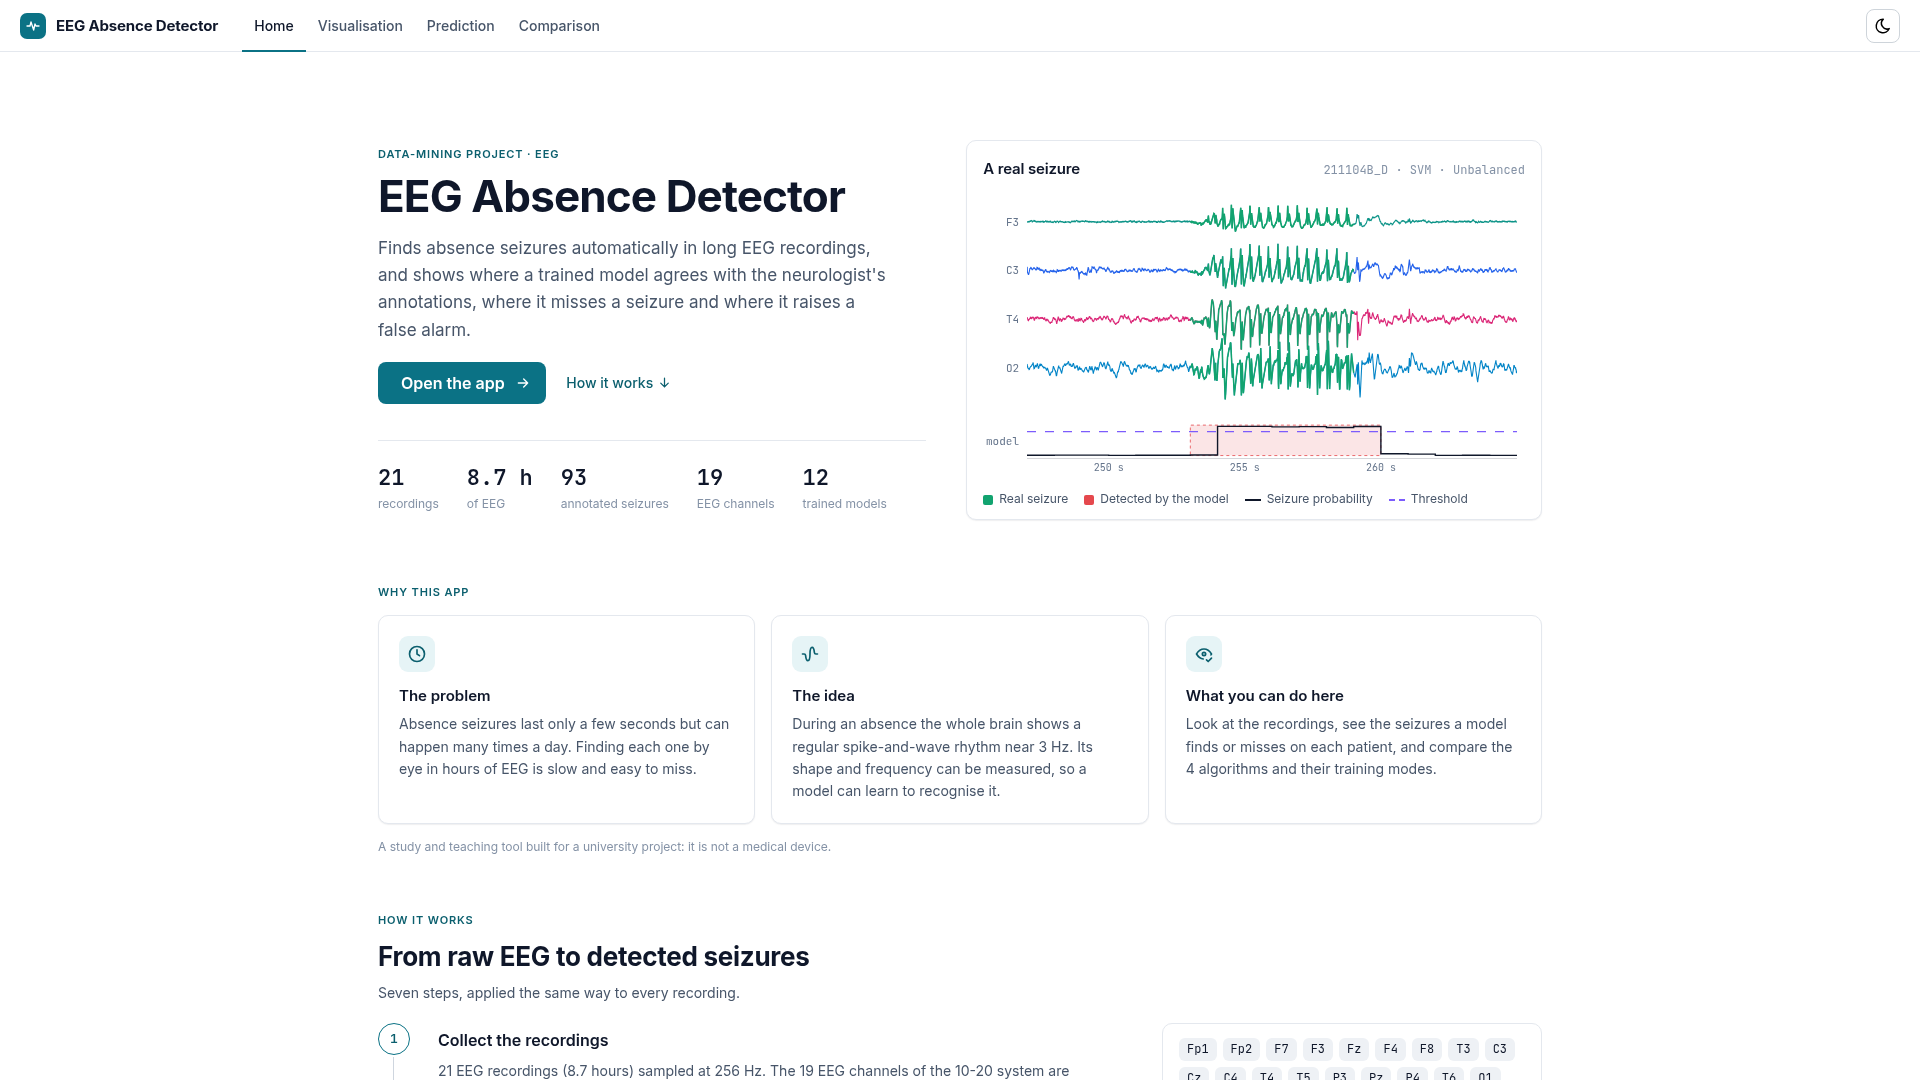
\includegraphics[width=\linewidth]{app/home_light_1920.png}
    \caption{Home}
  \end{subfigure}
  \hfill
  \begin{subfigure}[b]{0.48\linewidth}
    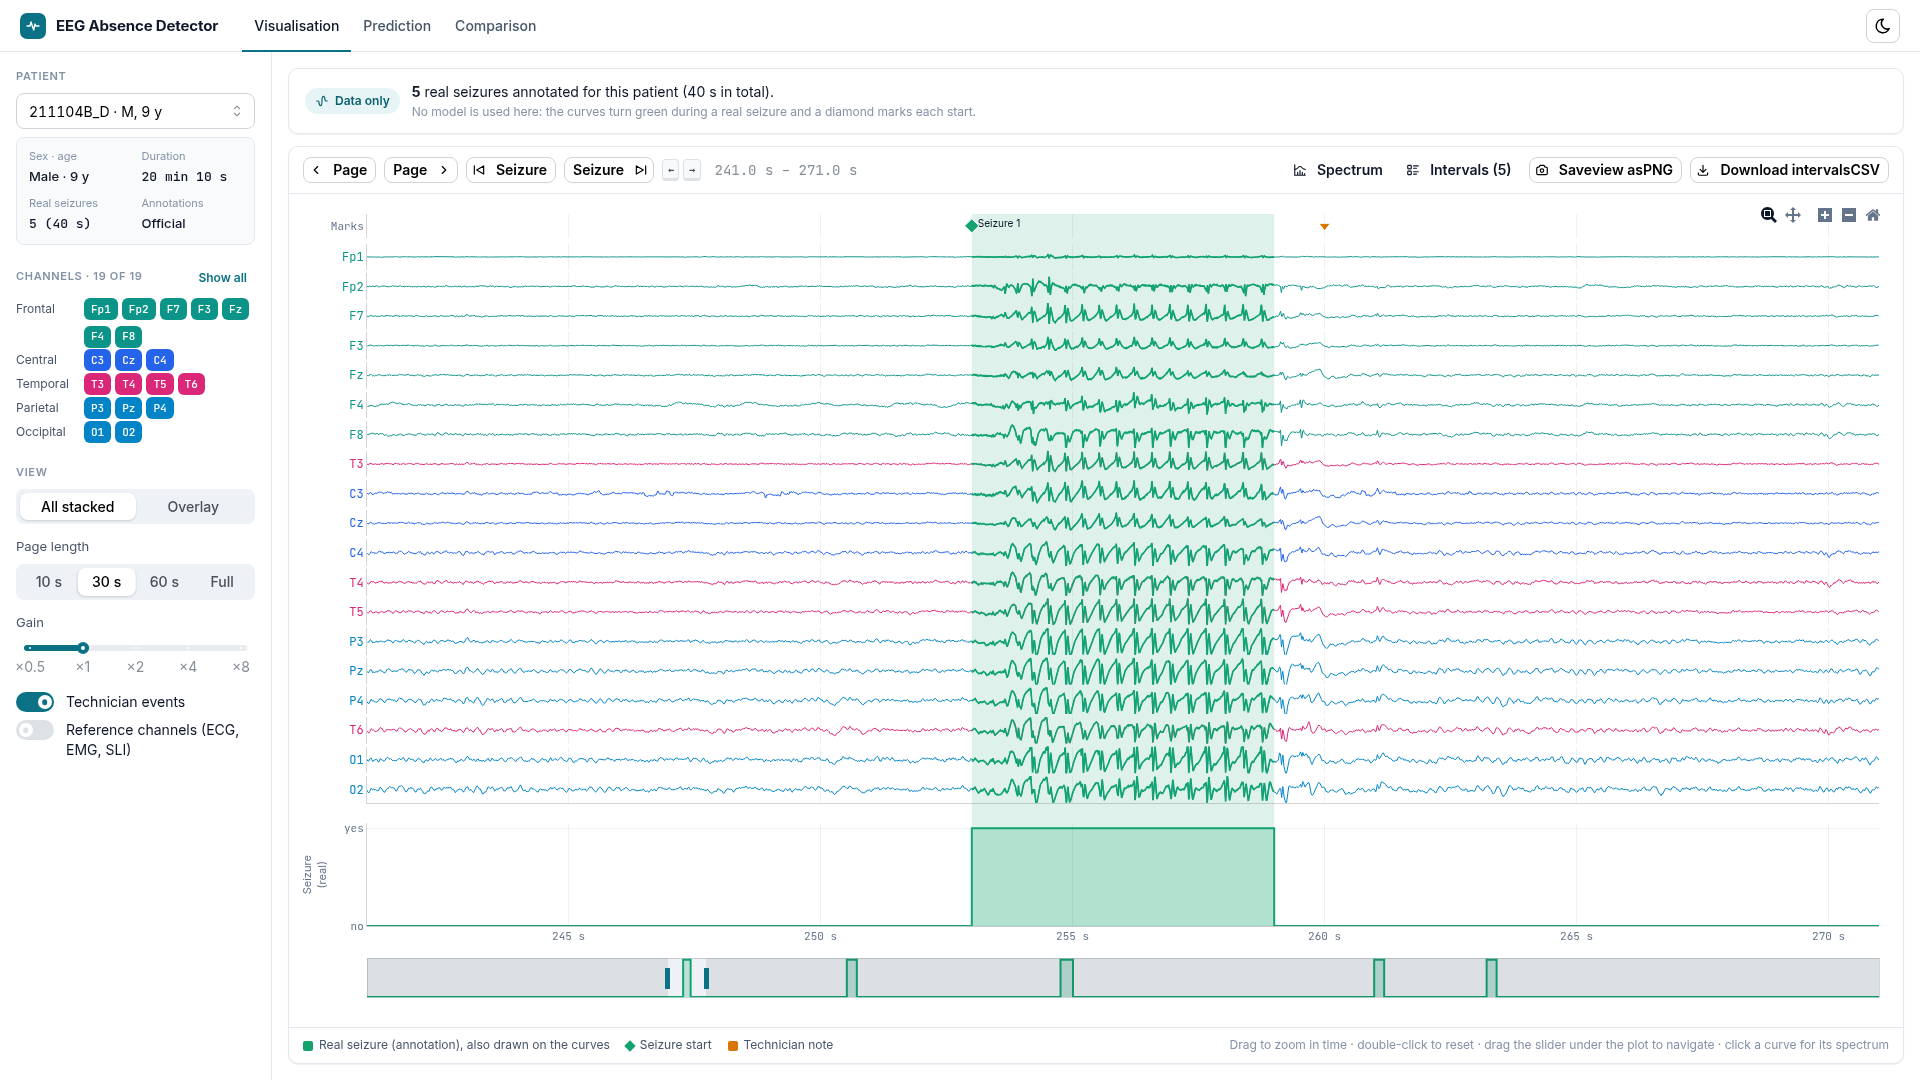
\includegraphics[width=\linewidth]{app/visualisation_light_1920.png}
    \caption{Visualisation}
  \end{subfigure}
  \caption{The Home and Visualisation pages, light theme.}
  \label{fig:app-home-vis}
\end{figure}

\section{Inspecting one patient closely}

The Prediction page is where a single detection can be examined in detail: pick a patient, pick
a model, pick a threshold, and the app shows exactly where that model's probability crosses the
line, against the real annotated seizure and the raw signal underneath it.

\begin{figure}[H]
  \centering
  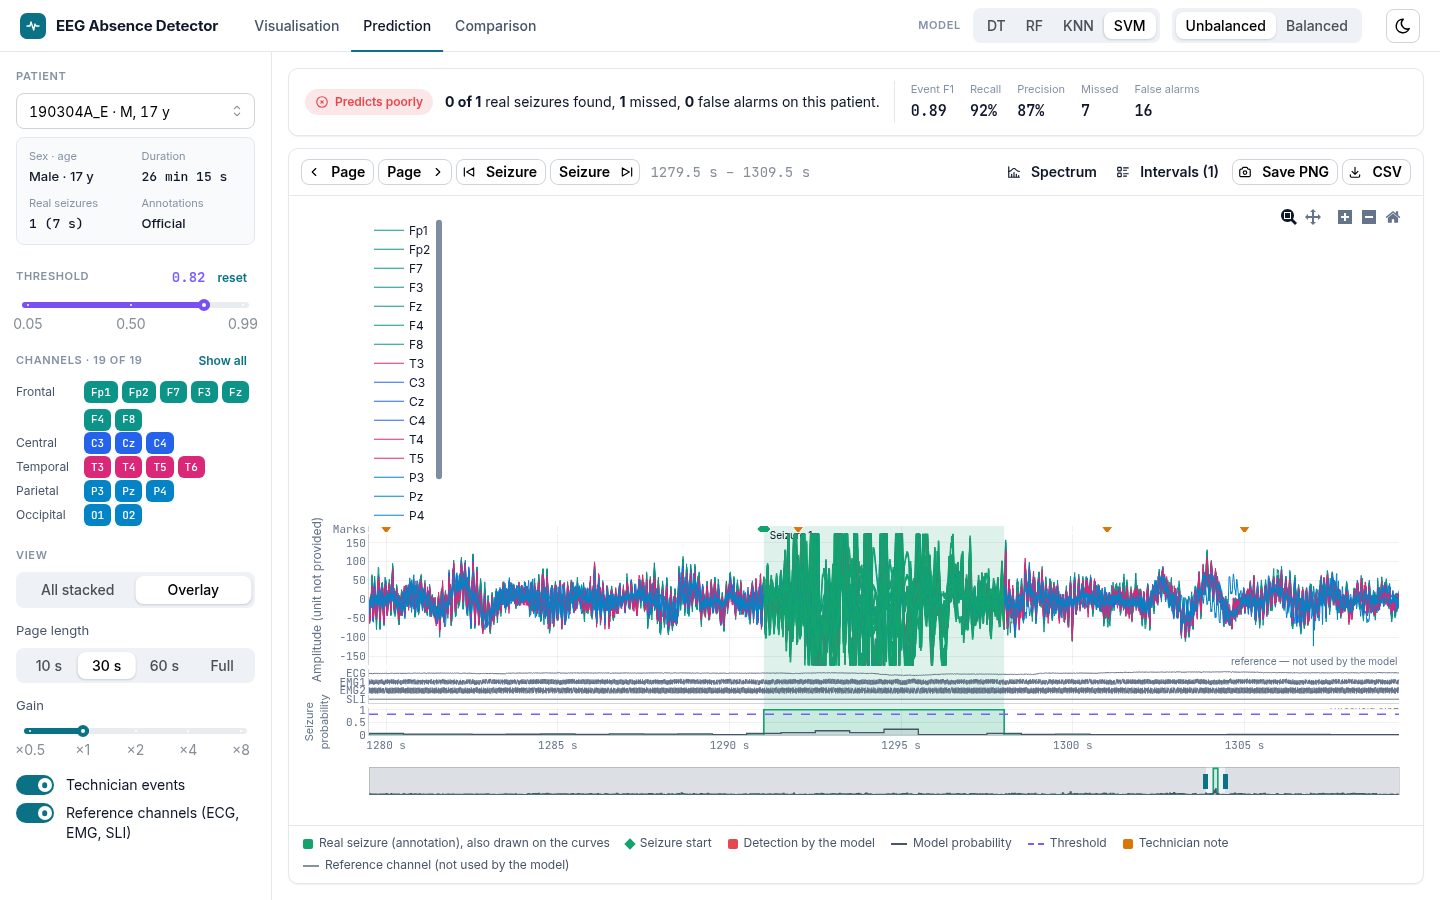
\includegraphics[width=0.92\linewidth]{app/state_overlay_1440.png}
  \caption{Patient \texttt{190304A\_E} on the Prediction page, overlay view: all 19 channels
    drawn on top of one another, with the seizure probability curve and threshold line
    underneath. This is a patient the SVM gets wrong --- the banner reads ``predicts poorly, 0
    of 1 real seizures found'' --- even though the model's numbers across all 21 recordings
    (\Cref{chap:classicalml}) are strong. The real seizure is highlighted in green on both the
    signal and the probability track: the model's probability visibly rises during the event but
    never crosses the 0.82 threshold, the same near-miss pattern already seen in
    \Cref{fig:error-examples}.}
  \label{fig:app-prediction-overlay}
\end{figure}

\section{A calm, clinical design}

The application went through a deliberate visual redesign, moving from its first working
version to a lighter, calmer default theme intended to feel appropriate for a clinical tool
rather than a generic data-science dashboard. The light theme uses a soft, slightly cool
background, white panels, dark slate text, and a single teal accent color; a parallel dark theme
follows the same structure. The 19 EEG channels are colored consistently by scalp region across
both themes.

\begin{figure}[H]
  \centering
  \begin{subfigure}[b]{0.48\linewidth}
    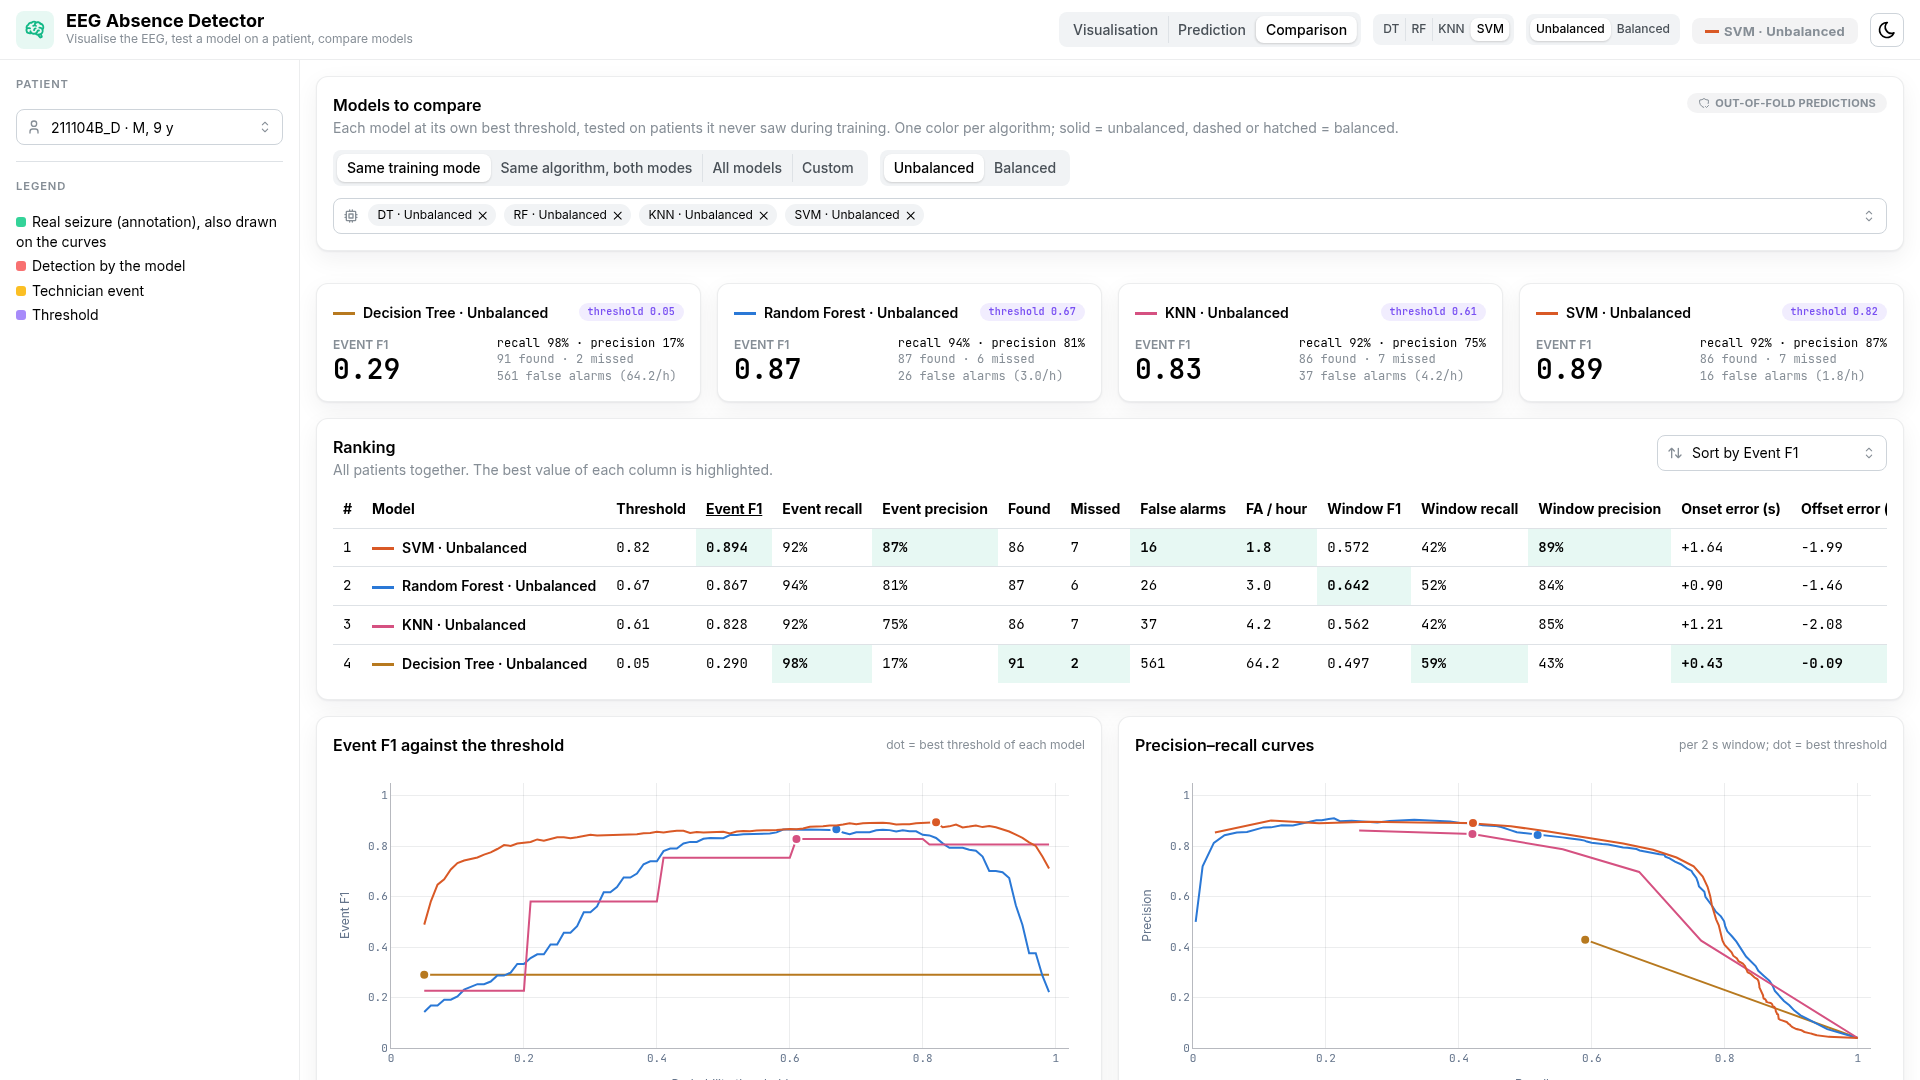
\includegraphics[width=\linewidth]{app/before/comparison_light_1080.png}
    \caption{Before}
  \end{subfigure}
  \hfill
  \begin{subfigure}[b]{0.48\linewidth}
    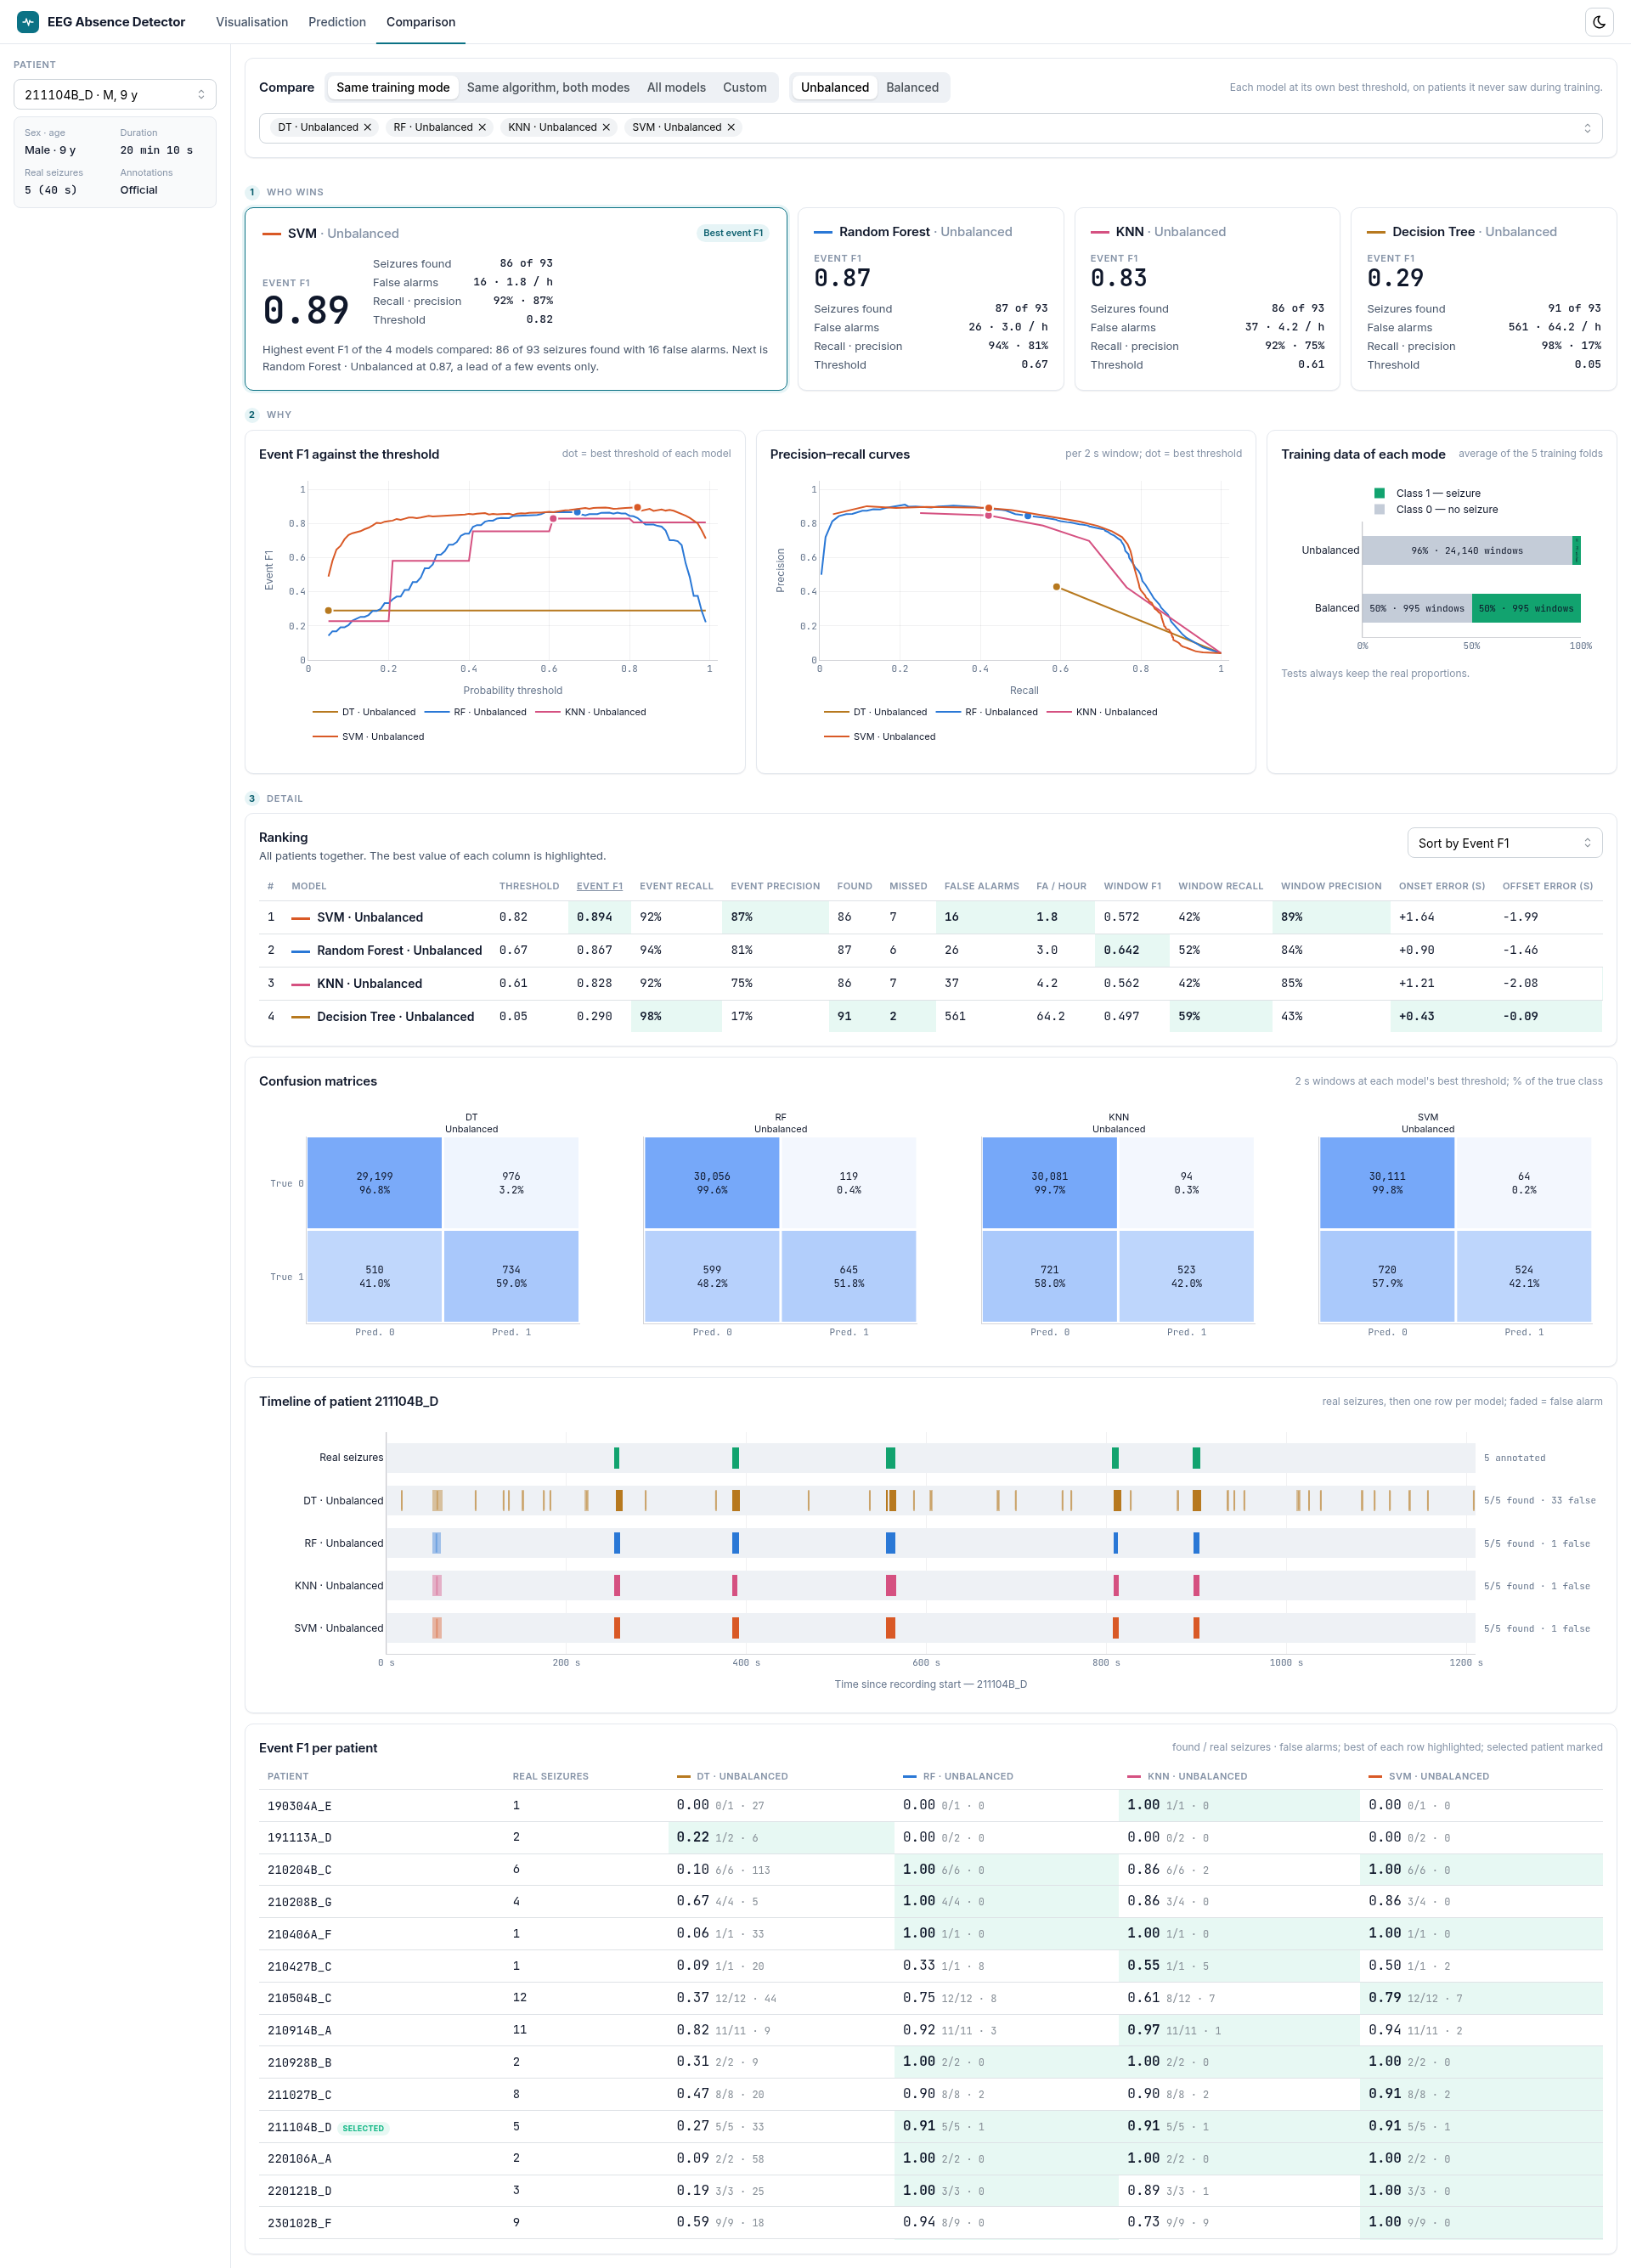
\includegraphics[width=\linewidth]{app/comparison_light_1920.png}
    \caption{After}
  \end{subfigure}
  \caption{The Comparison page before and after the redesign: a denser, plain-gray dashboard
    became a calmer, more explained one, with the same underlying numbers.}
  \label{fig:app-before-after}
\end{figure}

\section{The Comparison page in depth}

The Comparison page's ``all models'' view puts every one of the 12 classical models side by
side for one chosen patient.

\begin{figure}[H]
  \centering
  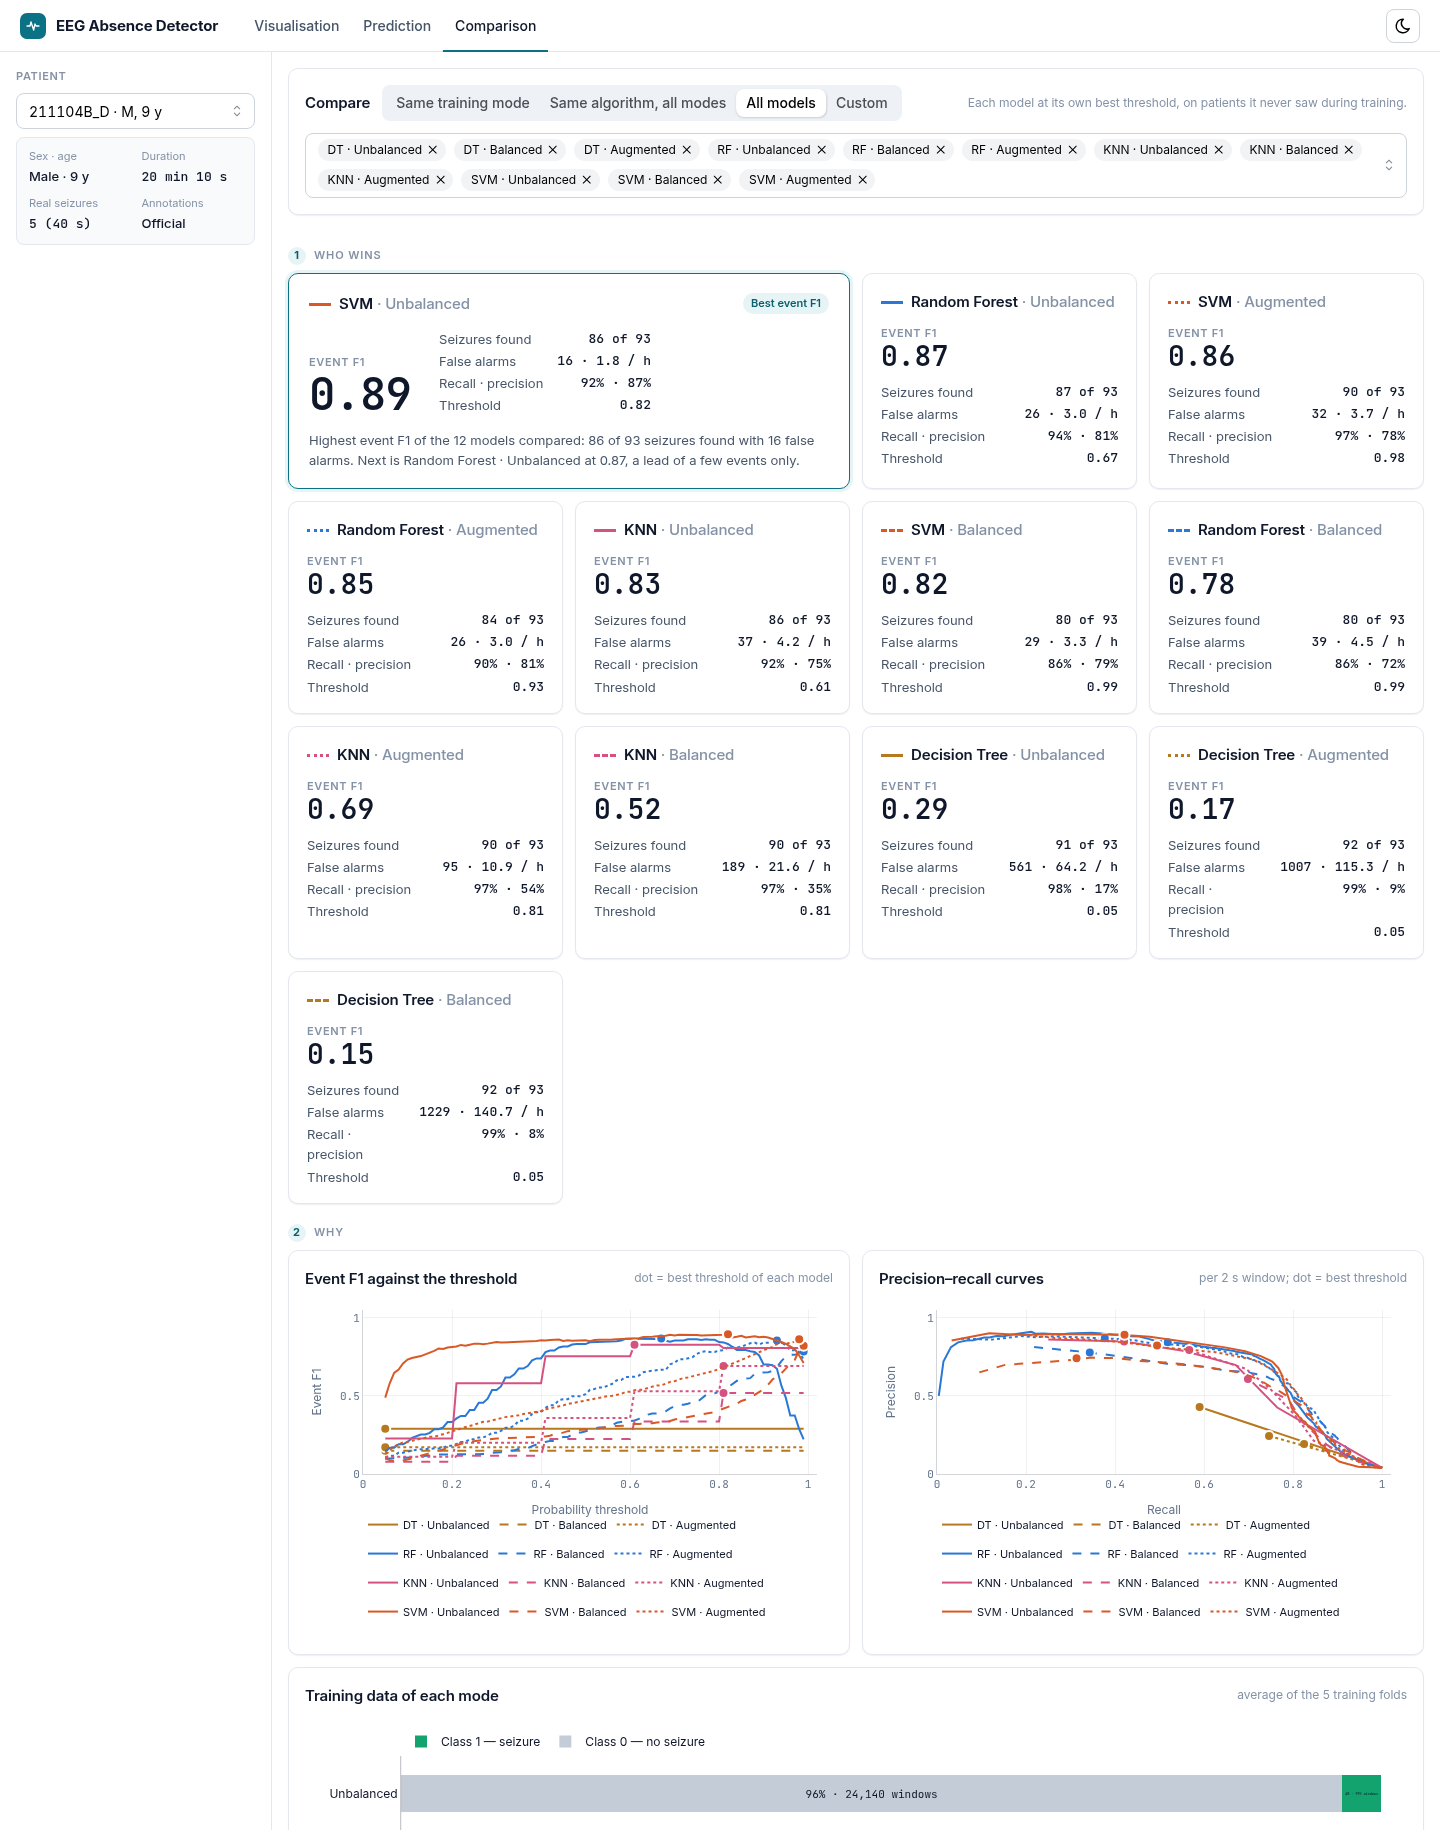
\includegraphics[width=0.92\linewidth]{comparison_depth_a.png}
  \caption{All 12 models selected for patient \texttt{211104B\_D}, each shown as a card with its
    event F1, seizures found, false alarms, recall, precision, and threshold --- SVM unbalanced
    is marked ``Best event F1.'' These numbers (0.89 event F1, 86 of 93 found, 16 false alarms,
    threshold 0.82) match \Cref{tab:classical-results} exactly, since the app reads the same
    underlying results rather than recomputing anything.}
  \label{fig:app-comparison-a}
\end{figure}

\begin{summarybox}
A four-page Dash application --- Home, Visualisation, Prediction, Comparison --- reads only
precomputed results and lets a visitor explore the real EEG signal, a chosen model's detections
down to a single missed seizure on a single patient, and a full 12-model comparison, in a
redesigned, calm clinical visual style. Every number shown in the app traces back to the exact
same results tables used throughout this report.
\end{summarybox}
